\documentclass{life-fr}
\usepackage{eurosans}
\usepackage{totpages}

\begin{document}

\title{La Vie est un Jeu}
\subtitle{Cahier des charges}
\member{Lepage Barbara}{db0company@gmail.com}
\member{Caradec Guillaume}{guillaume.caradec@gmail.com }
\member{El-Outmani Youssef}{youssef.eloutmani@gmail.com}
\member{Glorieux François}{fra.glorieux@gmail.com}
\member{Klarman Nicolas}{nickoas@gmail.com}
\member{Lassagne David}{david.lassagne@gmail.com}
\member{Le-Cor Wilfried}{wilfried.lecor@gmail.com}
\member{Lenormand Frank}{lenormf@gmail.com}
\member{Louvigny Guillaume}{guillaume@louvigny.fr}

\summary
{
  Le cahier des charges vise à définir simplement les « spécifications de base » de notre service à réaliser.
}

\maketitle

\chapter*{Résumé}
{
  Le présent cahier des charges est un document contractuel visant à définir les spécification de La Vie est un Jeu, notre EIP.\\
  Il précise l'ensemble des fonctionnalités, en plus de l'architecture du site et des applications mobiles.\\
  La structure interne de la base de données sera également décrite.\\
  Ce document détaillera également les cibles potentielles du projet et tentera d'estimer les contraintes financière et temporelles nécessaire pour mener à bien la réalisation de ce projet.\\
  Enfin l'ouverture offerte aux programmeurs tiers sera également abordée.\\
}

\chapter*{Informations du document}

\begin{tabular}{ | m{5cm} | m{10cm} | }
  \hline
  Type du document & Cahier des Charges\\
  \hline
  Nom du groupe & La Vie Est Un Jeu\\
  \hline
  Nombre de pages & \ref{TotPages} \\
  \hline
  Titre complet du document & Cahier des Charges du projet ``La Vie Est Un Jeu''\\
  \hline
  Auteurs & Membres du groupe, voir page de garde\\
  \hline
  Responsable & Chef de groupe : Barbara Lepage\\
  \hline
  Contact & lavieestunjeu@googlegroups.com\\
  \hline
  Mots clés & ``cahier des charges'', ``lavieestunjeu''\\
  \hline
  Révision actuelle & 1.8\\
  \hline
  Site vitrine & http://eip.epitech.eu/2014/lavieestunjeu/\\
  \hline
  Site officiel & Non disponible\\
  \hline
\end{tabular}

\chapter*{Table des révisions}

\revision{1.0}{Lepage Barbara}{Rappel de l'EIP}{05/04/2012}
\revision{1.1}{Louvigny Guillaume}{Principe de base du système futur}{05/04/2012}
\revision{1.2}{Lepage Barbara}{Environnement matériel}{05/04/2012}
\revision{1.3}{Lenormand Frank}{Environnement de réalisation}{05/04/2012}
\revision{1.4}{Lenormand Frank}{Architecture technique}{05/04/2012}
\revision{1.5}{Klarman Nicolas}{Gestion de la sécurité}{05/04/2012}
\revision{1.6}{Lepage Barbara}{Points sensibles}{05/04/2012}
\revision{1.7}{Le-Cor Wilfried}{Description des tests de premier niveau}{05/04/2012}
\revision{1.8}{Lassagne David}{Schéma de la base de données}{05/04/2012}
\listofrevisions

\newpage
\hspace{2cm}
\newpage

\tableofcontents

\newpage
\hspace{2cm}
\newpage

\chapter{Rappel de l'EIP}
\section{Qu'est-ce qu'un EIP et Epitech}
Epitech est une école formant des experts en informatique. Sa pédagogie par projets implique directement les étudiants dans leur apprentissage et les rend plus à même de réagir et s'adapter aisément, par exemple aux évolutions technologiques qui auront lieu au cours de leur carrière.\\

Un Epitech Innovative Project ou EIP est l'élément clé du cursus Epitech. Il s'agit d'un projet de fin d'études regroupant un minimum de six étudiants autour d'un but commun. Ce projet est conduit sur une durée de trois ans, beaucoup plus importante que celles des projets réalisés lors des trois premières années d'études. De plus, l'EIP amène les étudiants à se confronter au monde de l'entreprise.

\section{Sujet de « La vie est un Jeu »}
Dans le cadre de notre EIP, nous avons décidé de réaliser un réseau social à but ludique basé sur les « bucket lists ». Une bucket list est « une liste de choses à faire avant de mourir » : elle définit toutes les choses que son auteur désire faire de son existence, une sorte de mémo pour ne pas gâcher sa vie. Notre projet permettra à nos visiteurs de construire leurs propres listes et de faire valider leurs exploits tout en les partageant avec leurs réseaux sociaux. Ainsi, chaque action réalisée par un utilisateur (ajout d'une activité, succès ou échec) sera un fil de discussion dans lequel le visiteur et son réseau pourra discuter et partager différents types de médias (photos, vidéos, etc.). L'activité d'un utilisateur sera validée par son propre réseau et apparaîtra sous forme de « succès », comme dans un jeu vidéo. Le site s'étendra par la suite en proposant d'autres caractéristiques propres aux jeux vidéo.

\section{Principe de base du système futur}

Vous présenterez une vue générale de votre projet tel qu’il doit être fonctionnellement, la cible quand il sera achevé. Quels sont vos objectifs, le domaine dans lequel il s’inscrit, pour qui et pour quoi il est réalisé. Vous vous baserez sur l’étude de l’existant pour construire cette partie.\\

Les utilisateurs ciblés par le projet sont très nombreux. Il suffit qu'une personne ait un centre d'intérêt ou une passion couvert(e) par le site pour qu'elle ait une raison de s'y inscrire. Le site comme les applications mobiles seront conçus en vue d'une internationalisation étendue.\\

Pour les utilisateurs finaux le projet sera composé d'un site web et de plusieurs applications mobiles incluant Android, iOS et Windows Phone. Pour les développeurs tiers, une API sera créée permettant la création de nouveaux usages.\\

L'EIP est créé pour pouvoir répondre à un ensemble de fonctionnalités non présentes dans les projets déjà existants. Ces fonctionnalités ne sont pas combinées ou présentes sur les sites concurrents. En effet, nous tenons à mettre en place une plate-forme suffisamment ludique pour être visitée au quotidien, sans pour autant négliger l’aspect social permettant au visiteur de discuter de ses loisirs avec son réseau et de pouvoir partager aisément ses expériences à travers photos et vidéos.\\

À l'issue de la première année de travail sur le projet en partenariat avec l'INRIA et le Koalab Epitech, nous estimons avoir un site fonctionnel. Pendant la seconde année de travail sur l'EIP nous aimerions pouvoir signer des partenariats commerciaux avec divers acteurs de domaines culturels ou encore événementiels. Cette période sera également l'occasion d'ajouter de nouvelles fonctionnalités annexes répondant à des besoins émanant par exemple des utilisateurs.

\section{But et destinataires du projet}

Le projet a pour but de créer une communauté d'utilisateurs autour d'un système d'« achievements », directement lié à la vie quotidienne, aux passions ou à la vie professionnelle.\\

Les utilisateurs ciblés sont très nombreux. En théorie, toute personne ayant un centre d'interêt ou une passion est une cible.\\

À plus long terme, des partenariats commerciaux permettront de cibler des marques et des lieux.\\

Le site sera multilingue, donc ouvert à l'internationalisation.

\section{Qu'est-ce qu'un ``Achievement'' ?}
Le terme achievement (qui peut être traduit par succès ou réalisation en français) est, dans le cadre vidéo-ludique,  un objectif défini à accomplir par le joueur, en dehors de l’objectif principal (c’est-à-dire, gagner ou finir le jeu).\\
 Les achievements sont donc des récompenses honorifiques ajoutant du challenge pour le joueur.\\
\\
Nous pourrions utiliser une traduction française du terme achievement mais nous pensons que achievement est le terme le plus populaire dans le monde video-ludique.\\
\\
Les achievements permettent au joueur de découvrir plus en profondeur le contenu du jeu et donc d’explorer de nouveaux horizons.\\
 L’obtention est souvent un moment agréable pour le joueur.\\
 Il ressent une certaine satisfaction et se sent récompensé pour un effort.\\
 Il peut ensuite les partager avec ses amis afin de recueillir les honneurs ou de défier ses amis de faire autant ou mieux, ce qui améliore grandement l’immersion au sein du jeu.\\
\\
Nous pensons, qu’il est intéressant d’en faire une analogie avec la vie.\\
 La vie est un jeu comme un autre et mérite d’avoir elle aussi ses achievements.\\

\newpage
\hspace{2cm}
\newpage


\chapter{Présentation de l’environnement de réalisation}

\section{Environnement matériel}

Notre projet tourne sur un serveur Ocsigen. Il est installé sur une Dedibox PRO Dell financée par les membres du projet.

\vspace{20pt}

\begin{tabular}{|c|c|}
  \hline
   Serveur & Dell® PowerEdge R210\\
  \hline
  Processeur & 1x Intel® Xeon® L3426\\
  \hline
  Architecture & 4x 1.86GHz, 64 Bits, Virtualisation\\
  \hline
  Mémoire vive & 16 Go DDR3 ECC\\
  \hline
  Disque dur & 2 x 2 To SATA2 Raid 0 / Raid 1 HARD (H200)\\
  \hline
  Prix mensuel & 49,99 euros HT\\
  \hline
\end{tabular}

\vspace{20pt}

\section{Coûts}

\begin{itemize}
  \item Un compte développeur pour chaque boutique d'application (iOS : AppStore (99\$), Google Play (Android : 25\$) et Marketplace Windows Phone (99\$)) pour les applications mobiles.
  \item Un serveur dédié, dans un premier temps taillé pour le développement du site pouvant gérer seulement peu d'utilisateurs connectés en même temps à environ 60 euros par mois.
  \item Un serveur de production, qui sera utilisé ultérieurement pouvant aller jusqu'à 600 euros par mois.
  \item Nous envisageons par la suite, une fois l'application complétement terminée, d'engager un graphiste pour les « achievements ».
\end{itemize}

\section{Environnement de réalisation}

Afin de communiquer et d’échanger sur le projet, notre groupe de travail s’appuie sur plusieurs outils.

\begin{itemize}
  \item En effet, LaVieEstUnJeu dispose de son canal IRC officiel (\#life-eip sur irc.epitech.net), dont le but est d’assurer un support rapide aux utilisateurs et contributeurs en gérant une historique des discussions.
  \item Additionnellement, l’équipe du projet a accès à une mailing list (hébergée par google groups).
  \item Elle gère tous les documents relatifs à l’évolution du projet grâce aux google documents.
  \item La documentation se trouve sur le site vitrine : \url{http://eip.epitech.eu/2014/lavieestunjeu/}
  \item Nous avons un bug tracker, un wiki et des tickets sur un dépôt privé GitHub.
\end{itemize}

\section{Architecture technique}

\begin{itemize}
  \item LaVieEstUnJeu se base sur un environnement Web en OCaml, donc la composante principale est le serveur web \href{http://ocsigen.org/}{Ocsigen}.
  \item Le projet s’appuiera également sur \href{http://ocsigen.org/js_of_ocaml/}{js\_of\_ocaml}, un outil de compilation d’OCaml en JavaScript.
  \item Il gèrera une base de données grâce à \href{http://ocsigen.org/macaque/}{Macaque}, un autre projet initié par l’INRIA.
\end{itemize}

\section{Gestion de la sécurité}

\begin{itemize}
  \item Mise en place d’une solution de « niveau de confidentialité », un utilisateur pourra définir un niveau de confidentialité pour chaque utilisateur de son réseau. 

\begin{figure}[H]
  \begin{center}
    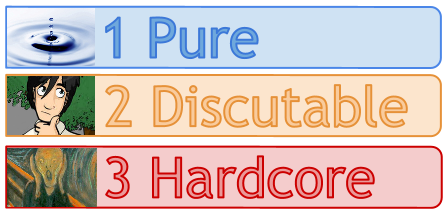
\includegraphics[width=10cm]{img/confidentialite.png}
  \end{center}
\end{figure}

\end{itemize}

\section{Points sensibles}

\begin{itemize}
  \item La sécurité des informations est une priorité pour nous. Nous ferons donc très attention à ce que les utilisateurs sachent toujours à tout moment qui a accès à quelles informations.
  \item Nous souhaitons conserver notre idée secrète jusqu’à ce que nous ayons une version de base utilisable.
\end{itemize}

\chapter{Description des différentes parties du programme à réaliser}

\section{Le Site Web}

\subsection{Vue d'ensemble de la page d'accueil avant le login}

L'utilisateur verra en premier lieu un diaporama mettant en avant certains « achievements », classés par date de publication et par popularité, ainsi que les diverses fonctions du site. Ce diaporama aura pour but d'inciter à l'utilisateur à procéder à son inscription.\\

La page d'accueil permettra également à l'utilisateur de s'inscrire au site. Cette inscription est détaillée plus loin.\\

La dernière fonctionnalité principale de cette page d'accueil est la connexion de l'utilisateur au site.\\

L'entrée du site pourrait éventuellement permettre de rechercher les « achievements » et catégories de celui-ci.

\subsection{L'inscription, les cinq premières minutes !}

L'objectif de cette étape serait clairement d'éviter toute la lourdeur que représente la récolte d'informations que le site a besoin d'effectuer auprès du futur utilisateur (présenter un formulaire compact et sauvage a des chances de rebuter celui-ci et éventuellement de le faire renoncer à son inscription).\\

Nous avons donc pensé à un système en mode pas à pas qui, tout en faisant découvrir notre outil et son univers à l'internaute, lui ferait de subtiles demandes d'informations de façon régulière, et ce afin d'alléger cette étape essentielle qui nous permettra de catégoriser le nouvel inscrit et de lui proposer du contenu en fonction de ces informations qui auront été récoltées.\\

En plus de combiner le rôle de « guide » pour la découverte du site et de « sondeur » pour la récolte d'informations, cette méthode a pour avantage de pousser l'utilisateur à aller au bout de la présentation, et donc de l'inscription, au fur et à mesure de son avancée (effet psychologique, il veut finir ce qu'il a commencé, puisqu'il a déjà commencé à contribuer, autant aller jusqu'au bout). La présentation allant, l'intérêt croissant, les chances d'une inscription augmentent à l'arrivée.\\
\\

Dans l'état actuel on imagine comme première approche une question simple qui amène à faire une simple action en mode « vous êtes à un clic de rentrer dans notre univers » avec, par exemple, le choix du genre : Homme, Femme, Non précisé.

\begin{figure}[H]
  \begin{center}
    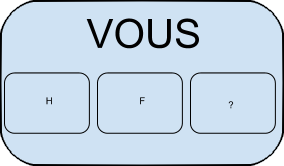
\includegraphics[width=10cm]{img/vous.png}
  \end{center}
\end{figure}

\subsection{La page d'accueil utilisateur une fois connecté}

La page d'accueil de l'utilisateur habitué au site présente son flux d'informations, à l'image des flux habituels de sites communautaires tels que Facebook ou Google+. \\

Le menu doit être discret. L'utilisateur doit tout de suite voir les quatre onglets principaux :

\begin{itemize}
  \item le flux (page d'accueil par défaut) ;
  \item les objectifs de l'utilisateur (ses inscriptions) ;
  \item les « achievements » ;
  \item les « amis » de l'utilisateur (importés des réseaux sociaux ou ajoutables dans le cadre du site).
\end{itemize}

Une barre de « breaking news » en permanence en haut du site donnera à l'utilisateur en une ligne les derniers « achievements » de ses amis ainsi que les nouveautés du site.

\begin{figure}[H]
  \begin{center}
    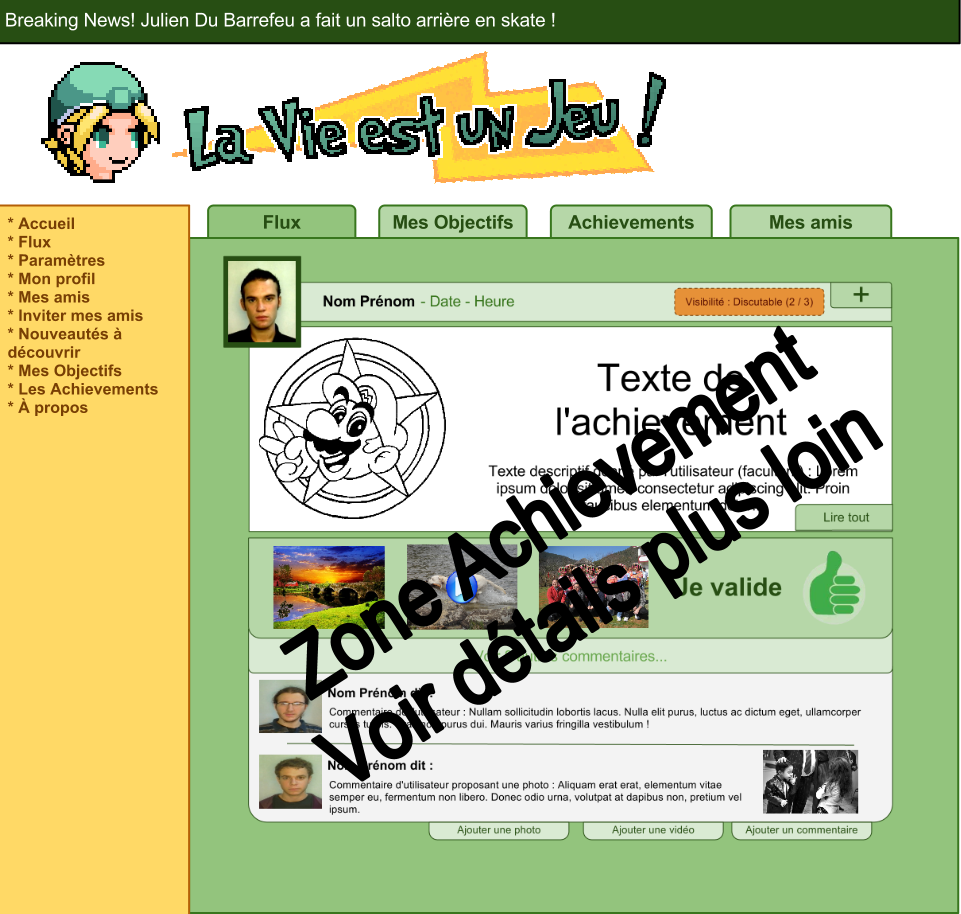
\includegraphics[width=15cm]{img/accueil.png}
  \end{center}
\end{figure}


\subsection{Onglet Flux (Feed)}

L'onglet Flux sera situé au milieu de la page principale et aura pour fonction d'afficher les derniers « achievements » à valider par le cercle d'amis.\\

Ce flux contiendra toutes les actions des contacts :

\begin{itemize}
  \item les « achievements » à valider (voir détails ci-dessous) ;
  \item les objectifs qu'ils se sont fixés ;
  \item les nouveaux contacts ;
  \item des nouveautés du site (informations ou nouveaux « achievements »).
\end{itemize}

\subsection{Détails d'un « achievement »}

Chaque « achievement » disposera d'une fonction Like qui permettra aux utilisateurs d'indiquer qu'ils aiment la publication en question, ainsi que d'un module d'envoi de preuves d'« achievements » servant à la validation. Le support de validation pourra être au format texte, photo ou vidéo. La photo de l'utilisateur apparaîtra ainsi que la description de l'« achievement », en regard de celle-ci. Il sera également possible de poster des commentaires en-dessous des preuves de validation. Un onglet « Plus » permettra de dérouler chaque « achievement » afin d'obtenir plus d'informations.\\

\begin{figure}[H]
  \begin{center}
    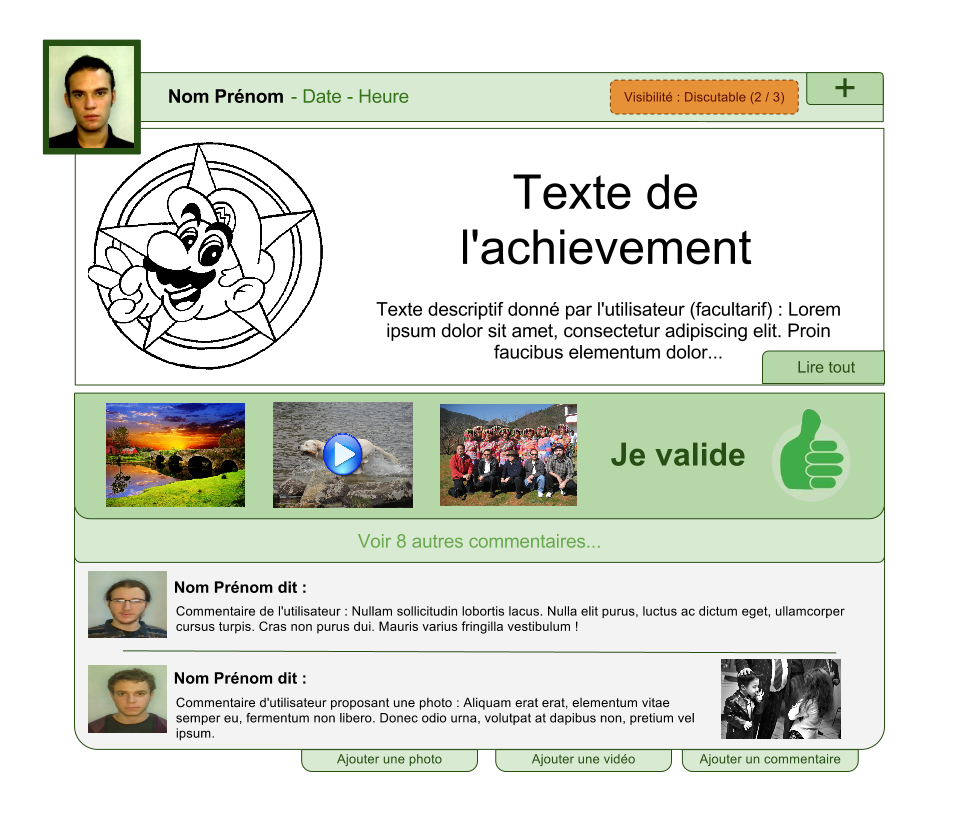
\includegraphics[width=15cm]{img/achievement.png}
  \end{center}
\end{figure}

\subsection{Onglet Achievements}

L'utilisateur pourra sélectionner des packs qui contiendront les « achievements » à accomplir. Les packs seront tous disponibles et classés par thématiques dans une sous-catégorie, mais la plate-forme proposera d'abord à l'utilisateur des packs d'« achievements » correspondant aux centres d'intérêt de ce dernier, ou encore de sa tranche d'âge. Une fois un pack sélectionné, l'utilisateur peut aussi définir certains « achievements » comme étant ses objectifs, et ainsi notifier son réseau.

\subsection{Onglet Objectifs}

L'onglet Objectifs permet à l'utilisateur de construire une « to-do list » ou « bucket-list », le but étant de filtrer les « achievements » que l'utilisateur ne désire pas réaliser dans l'immédiat et ainsi de dégager ceux qu'il va accomplir sur le court terme. La page est destinée à être régulièrement consultée : c'est à partir de cet onglet que l'utilisateur peut annoncer la fin d'un objectif, et donc obtenir un « achievement » si ses amis confirment la validation de ce dernier.

\subsection{Onglet Contacts}

L'utilisateur pourra ici voir sa liste de contacts et les profils de ceux-ci, mais aussi regrouper ses contacts par groupe. Les groupes d'utilisateurs permettent alors d'attribuer des degrés de sensibilité.
Le degré de sensibilité va de 0 à 3 et permet de partager les « achievements » aux contacts de son choix.

\subsection{Page Profil}
La page Profil contient les informations d'un utilisateur, et permet de les modifier. Si l'utilisateur consulte la page profil d'un autre membre, il a la possibilité d'interagir avec lui de différentes manières (envoi de message, demande d'ajout en ami, ...).
La page profil contient principalement des badges d'« achievement », tel un tableau de chasse. L'utilisateur peut cliquer sur l'« achievement » pour en avoir le détail (textes, photos, vidéos, commentaires).

\section{L'application Smartphone}
Pour ce qui est des smartphones, nous avons décidé de ne pas coder dans les langages propres à chaque plate-forme, mais de développer une interface sur la base de la technologie que nous utilisons pour notre site web, à savoir Ocsigen. Cela nous permettra d'être constants dans notre ligne directrice de code. Cette interface sera chargée sur toutes les plates-formes smartphones sous forme d'une Web-view. L'avantage de cette méthode réside dans sa totale portabilité qui nous évite d'avoir à développer une application spécifique à chaque plate-forme existante.

\section{L'API}

L'API permettrait d'offrir aux développeurs un accès à l'essentiel des fonctionnalités du site. On pourra y récupérer, pour un utilisateur donné, et selon les vœux de celui-ci (token d'acceptation), la liste de ses « achievements ».


\chapter{Description de la base de données}

\section{Description des tests de premier niveau}

\begin{itemize}
  \item{Creation de compte}
  \item {Restriction d’accès par cercles}
  \item Listing des « achievements » déja présents dans la base de données.
  \item Sélection d’« achievements » parmi ceux disponibles.
  \item Pondération des « achievements ».
  \item Classement : tests des différents algorithmes de notation.
  \item Restriction des achievements pour une catégorie d’utilisateurs (ceux de niveau 3 ne seront pas accessibles au moins de 18 ans et ceux de niveau 2 aux moins de 14 ans).
\end{itemize}

\section{Schéma de la base de données}

\begin{figure}[H]
  \begin{center}
    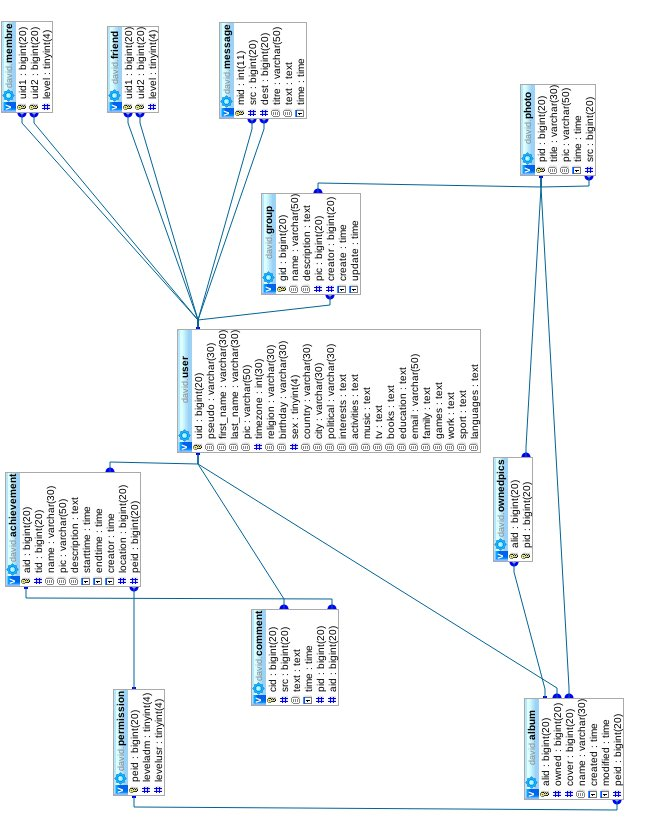
\includegraphics[width=18cm]{img/imgdb.jpg}
  \end{center}
\end{figure}

\chapter{Organisation projet}

\section{Planning}

D'un point de vue global, le projet se déroulera en trois grandes parties : documentation, développement et mise en production.\\

Avant de passer à la réalisation concrète du produit, nous allons nous consacrer à la rédaction de plusieurs documents essentiels au bon déroulement du projet. En effet, il est nécessaire de définir précisément les détails du projet, étudier les différents outils et technologies à notre disposition et faire des choix, ou encore mettre en place des partenariats. Nous continuerons cette étude jusqu'en septembre 2012.\\

Une fois les outils en main, les spécificités définies et les rôles attribués, nous commencerons à développer le produit. Nous pensons mettre en ligne une version Bêta pour septembre 2013.\\

La dernière période sera consacrée aux problématiques de communication, et dans une moindre mesure de développement. Ainsi, durant la dernière année du projet, nous tâcherons de faire connaître ce dernier de diverses façons, pour créer la communauté indispensable à notre plate-forme, en plus de la finalisation technique du produit. Nous pourrons de ce fait bénéficier de retours d'utilisateurs, afin de corriger les anomalies et peaufiner la plate-forme.

\section{Équipe}

Durant la période de développement du produit, l'équipe sera dispersée dans plusieurs pays, rendant tout travail en équipe difficile. Nous allons nous répartir les tâches de manière à pouvoir travailler de façon relativement autonome : notre projet étant composé de plusieurs éléments distincts, nous nous arrangerons pour ne pas en partager un entre des membres situés dans des lieux différents.\\

Au niveau de la répartition des rôles: Guillaume Caradec s'occupe de la gestion de projet, et Barbara Lepage dirige la partie technique. Nous sommes bien évidemment tous à la charge du développement et de la rédaction de la documentation.\\

Nous avons à notre disposition divers outils pour nous organiser et communiquer plus facilement :\\

\begin{itemize}
  \item une mailing-list et un canal IRC, permettant de traiter l'ensemble des diverses problématiques ;
  \item un dossier Google Docs, pour pouvoir partager les documents liés au projet et leur rédaction ;
  \item Gtalk, une application de Google permettant d'organiser des visio-conférences via un navigateur ;
  \item un dépôt Git ;
  \item l'utilisation de Doodle, pour planifier plus facilement les réunions.
\end{itemize}

Les membres du groupe se réuniront toutes les semaines pour parler de l'avancement du projet, des imprévus rencontrés et des objectifs à court terme.

\section{Planning détaillé avec dates précises}

Veuillez vous reporter au fichier joint \texttt{2014\_GAN\_FR\_lavieestunjeu.pdf}. Il contient le diagramme de Gantt de notre projet.


\newpage
\hspace{2cm}
\newpage


\chapter{Conclusion}


Ce document présentait donc les spécification de notre EIP, La Vie est un Jeu.\\
\\
Nous y avons décrit l'ensemble des fonctionnalités qui seront proposées, ce qui inclue à la fois le site web ainsi que les applications mobiles.\\
\\
Était également présenté la définition de la base de donnée applicable sur toutes les plates-formes visées.\\
\\
L’API à destination de développeurs tiers avait également été définie.\\
\\
Pour finir, il détaillait également ceux à qui se destine le projet, et estimait les diverses contraintes imposées par celui-ci qu’elles soient d’ordre financières ou organisationnelles.\\


\newpage
\hspace{2cm}
\newpage

\end{document}
